\chapter*{Dodatak: Prikaz aktivnosti grupe}
		\addcontentsline{toc}{chapter}{Dodatak: Prikaz aktivnosti grupe}
		
		\section*{Dnevnik sastajanja}
		
		\textbf{\textit{Kontinuirano osvježavanje}}\\
		
		 \textit{U ovom dijelu potrebno je redovito osvježavati dnevnik sastajanja prema predlošku.}
		
		\begin{packed_enum}
			\item  sastanak
			\item[] \begin{packed_item}
				\item Datum: 5. listopada 2020.
				\item Prisustvovali: G.Crnogorac, L.Ilić, M.Marfat, L.Nuić, B.Paradžik, M.Rašić, L.Srdarev
				\item Teme sastanka:
				\begin{packed_item}
					\item  sastanak a asistentom
					\item  objašnjenje zadatka
					\item  rasprava o predloženom zadatku
				\end{packed_item}
			\end{packed_item}
			
			\item  sastanak
			\item[] \begin{packed_item}
				\item Datum: 17. listopada 2020.
				\item Prisustvovali: G.Crnogorac, L.Ilić, M.Marfat, L.Nuić, B.Paradžik, M.Rašić, L.Srdarev
				\item Teme sastanka:
				\begin{packed_item}
					\item  rasprava o funkcionalnim zahtjevima i obrascima uporabe
					\item  razgovor o iskustvima pojedinih članova u različitim tehnologijama
				\end{packed_item}
			\end{packed_item}
			
			\item  sastanak
			\item[] \begin{packed_item}
				\item Datum: 19. listopada 2020.
				\item Prisustvovali: G.Crnogorac, L.Ilić, M.Marfat, L.Nuić, B.Paradžik, M.Rašić, L.Srdarev
				\item Teme sastanka:
				\begin{packed_item}
					\item  sastanak s asistentom 
					\item  dogovor o tehnologijama koje će se koristiti u projektu
				\end{packed_item}
			\end{packed_item}
			
			\item  sastanak
			\item[] \begin{packed_item}
				\item Datum: 28. listopada 2020.
				\item Prisustvovali: G.Crnogorac, L.Ilić, M.Marfat, L.Nuić, B.Paradžik, M.Rašić, L.Srdarev
				\item Teme sastanka:
				\begin{packed_item}
					\item  dogovor o daljnoj podjeli zadataka
					\item  rasprava o bazi podataka
				\end{packed_item}
			\end{packed_item}
			
			\item  sastanak
			\item[] \begin{packed_item}
				\item Datum: 5. studenoga 2020.
				\item Prisustvovali: G.Crnogorac, L.Ilić, M.Marfat, L.Nuić, B.Paradžik, M.Rašić, L.Srdarev
				\item Teme sastanka:
				\begin{packed_item}
					\item  povezivanje frontenda i backenda
					\item  detaljnija rasprava o bazi podataka
				\end{packed_item}
			\end{packed_item}	
			
			\item  sastanak
			\item[] \begin{packed_item}
				\item Datum: 9. studenoga 2020.
				\item Prisustvovali: M.Marfat, L.Nuić, M.Rašić, L.Srdarev
				\item Teme sastanka:
				\begin{packed_item}
					\item  sastanak s asistentom
					\item  pregled dosadašnjeg rada
				\end{packed_item}
			\end{packed_item}
		
			\item  sastanak
			\item[] \begin{packed_item}
				\item Datum: 2. prosinca 2020.
				\item Prisustvovali:  G.Crnogorac, L.Ilić, M.Marfat, L.Nuić, B.Paradžik, M.Rašić, L.Srdarev 
				\item Teme sastanka:
				\begin{packed_item}
					\item  sastanak s asistenticom - evaluacija dosadašnjeg rada
				\end{packed_item}
			\end{packed_item}
		
			\item  sastanak
			\item[] \begin{packed_item}
				\item Datum: 23. prosinca 2020.
				\item Prisustvovali:  G.Crnogorac, L.Ilić, M.Marfat, L.Nuić, B.Paradžik, M.Rašić, L.Srdarev 
				\item Teme sastanka:
				\begin{packed_item}
					\item  pregled napravljenog dijela projekta
					\item  plan nastavka projekta
					\item  podjela zadataka  
				\end{packed_item}
			\end{packed_item}
		
			\item  sastanak
			\item[] \begin{packed_item}
				\item Datum: 29. prosinca 2020.
				\item Prisustvovali:  G.Crnogorac, L.Ilić, M.Marfat, L.Nuić, M.Rašić, L.Srdarev, B.Paradžik
				\item Teme sastanka:
				\begin{packed_item}
					\item  pregled napravljenog od zadnjeg sastanka 
					\item  podjela novih zadataka za backend i frontend 
				\end{packed_item}
			\end{packed_item}
		
			\item  sastanak
			\item[] \begin{packed_item}
				\item Datum: 2. siječnja 2021.
				\item Prisustvovali:  G.Crnogorac, L.Ilić, M.Marfat, L.Nuić, M.Rašić, L.Srdarev 
				\item Teme sastanka:
				\begin{packed_item}
					\item  pregled napravljenog od zadnjeg sastanka 
					\item  podjela novih zadataka za backend i frontend
				\end{packed_item}
			\end{packed_item}
		
			\item  sastanak
			\item[] \begin{packed_item}
				\item Datum: 4. siječnja 2021.
				\item Prisustvovali: L.Ilić, L.Nuić, B.Paradžik, L.Srdarev
				\item Teme sastanka:
				\begin{packed_item}
					\item  pregled napravljenih funkcionalnosti backenda 
					\item  rješavanje dosadašnjih problema u implementaciji backenda
				\end{packed_item}
			\end{packed_item}
		
			\item  sastanak
			\item[] \begin{packed_item}
				\item Datum: 4. siječnja 2021.
				\item Prisustvovali: G.Crnogorac,  M.Marfat, L.Nuić, M.Rašić
				\item Teme sastanka:
				\begin{packed_item}
					\item  pregled napravljenih funkcionalnosti frontenda 
					\item  podjela novih zadataka za frontend
				\end{packed_item}
			\end{packed_item}
		
			\item  sastanak
			\item[] \begin{packed_item}
				\item Datum: 6. siječnja 2021.
				\item Prisustvovali: G.Crnogorac, L.Ilić, M.Marfat, L.Nuić, M.Rašić, L.Srdarev, B.Paradžik
				\item Teme sastanka:
				\begin{packed_item}
					\item  pregled napravljenih funkcionalnosti backenda 
					\item  pregled rada aplikacije
					\item  utvrđvanje i rješavanje
					 grešaka aplikacije
					\item  aktualizacija dokumentacije
				\end{packed_item}
			\end{packed_item}
		
			\item  sastanak
			\item[] \begin{packed_item}
				\item Datum: 7. siječnja 2021.
				\item Prisustvovali: G.Crnogorac, L.Ilić, M.Marfat, L.Nuić, M.Rašić, L.Srdarev, B.Paradžik
				\item Teme sastanka:
				\begin{packed_item}
					\item  sastanak s asistentom - demonstracija alfa inacice
				\end{packed_item}
			\end{packed_item}
		
			
			
			
			
			%
			
		\end{packed_enum}
		
		\eject
		\section*{Tablica aktivnosti}
		
			\textbf{\textit{Kontinuirano osvježavanje}}\\
			
			 \textit{Napomena: Doprinose u aktivnostima treba navesti u satima po članovima grupe po aktivnosti.}
					
						
			
			\begin{longtabu} to \textwidth {|X[7, l]|X[1, c]|X[1, c]|X[1, c]|X[1, c]|X[1, c]|X[1, c]|X[1, c]|}
								
				\cline{2-8} \multicolumn{1}{c|}{\textbf{}} &     \multicolumn{1}{c|}{\rotatebox{90}{\textbf{Lovro Nuić }}} & \multicolumn{1}{c|}{\rotatebox{90}{\textbf{Grgur Crnogorac }}} &	\multicolumn{1}{c|}{\rotatebox{90}{\textbf{Luka Ilić }}} &	\multicolumn{1}{c|}{\rotatebox{90}{\textbf{Marko Marfat }}} &
				\multicolumn{1}{c|}{\rotatebox{90}{\textbf{Berislav Paradžik }}} &
				\multicolumn{1}{c|}{\rotatebox{90}{\textbf{Marin Rašić }}} &	\multicolumn{1}{c|}{\rotatebox{90}{\textbf{Luka Srdarev }}} \\ \hline 
				\endfirsthead
				
			
				\cline{2-8} \multicolumn{1}{c|}{\textbf{}} &     \multicolumn{1}{c|}{\rotatebox{90}{\textbf{Lovro Nuić }}} & \multicolumn{1}{c|}{\rotatebox{90}{\textbf{Grgur Crnogorac }}} &	\multicolumn{1}{c|}{\rotatebox{90}{\textbf{Luka Ilić }}} &
				\multicolumn{1}{c|}{\rotatebox{90}{\textbf{Marko Marfat }}} &	\multicolumn{1}{c|}{\rotatebox{90}{\textbf{Berislav Paradžik }}} &
				\multicolumn{1}{c|}{\rotatebox{90}{\textbf{Marin Rašić }}} &	\multicolumn{1}{c|}{\rotatebox{90}{\textbf{Luka Srdarev }}} \\ \hline 
				\endhead
				
				
				\endfoot
							
				 
				\endlastfoot
				
				Upravljanje projektom 		& 10 &  &  &  &  &  & \\ \hline
				Opis projektnog zadatka 	&  &  &  &  & 2 & 3 & \\ \hline
				
				Funkcionalni zahtjevi       &  &  & 1 & 1 &  & 1 &  \\ \hline
				Opis pojedinih obrazaca 	&  &  & 1 & 1 &  & 1 &  \\ \hline
				Dijagram obrazaca 			&  & 4 &  &  &  &  &  \\ \hline
				Sekvencijski dijagrami 		&  &  &  & 3 &  &  &  \\ \hline
				Opis ostalih zahtjeva 		&  &  &  & 1 &  &  &  \\ \hline

				Arhitektura i dizajn sustava	 &  &  & 3 &  &  &  & 8 \\ \hline
				Baza podataka				&  &  & 4 &  &  &  & 10  \\ \hline
				Dijagram razreda 			& 10 &  &  &  &  &  &   \\ \hline
				Dijagram stanja				&  &  &  &  &  &  &  \\ \hline
				Dijagram aktivnosti 		&  &  &  &  &  &  &  \\ \hline
				Dijagram komponenti			&  & 1.5 &  &  &  &  &  \\ \hline
				Korištene tehnologije i alati 		&  &  &  &  &  &  &  \\ \hline
				Ispitivanje programskog rješenja 	&  &  & 12 &  &  &  & 12 \\ \hline
				Dijagram razmještaja			&  & 1.5 &  &  &  &  &  \\ \hline
				Upute za puštanje u pogon 		& 1 &  &  &  &  &  &  \\ \hline 
				Dnevnik sastajanja 			& 1 &  &  &  &  & 0.5  &  \\ \hline
				Zaključak i budući rad 		&  &  &  &  &  &  &  \\  \hline
				Popis literature 			&  &  &  &  &  &  &  \\  \hline
				&  &  &  &  &  &  &  \\  \hline
				&  &  &  &  &  &  &  \\ \hline \hline
				\textit{Backend} 	& 80 &  & 25 &  & 4 &  & 25 \\  \hline
				\textit{Frontend} 	&  & 45 &  & 35 &  & 40 &  \\  \hline
				 							&  &  &  &  &  &  &\\  \hline
				
				
			\end{longtabu}
					
					
		\eject
		\section*{Dijagrami pregleda promjena}

		\begin{figure}[H]
			\centering
			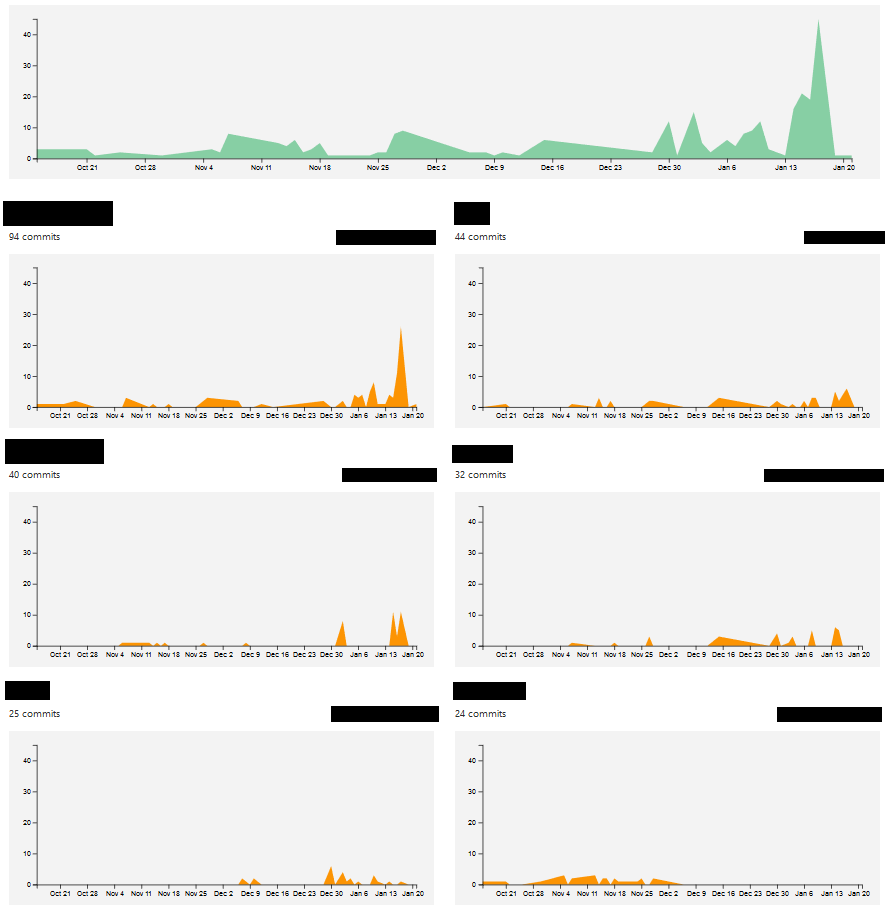
\includegraphics[scale=0.6]{slike/aktivnost.png}
			\caption{Dijagram pregleda promjena}
		\end{figure}
		
%		\textbf{\textit{dio 2. revizije}}\\
		
%		\textit{Prenijeti dijagram pregleda promjena nad datotekama projekta. Potrebno je na kraju projekta generirane grafove s gitlaba prenijeti u ovo poglavlje dokumentacije. Dijagrami za vlastiti projekt se mogu preuzeti s gitlab.com stranice, u izborniku Repository, pritiskom na stavku Contributors.}
		
	